\documentclass[10pt, a4paper]{report}

\usepackage[utf8]{inputenc}
\usepackage{polski}
\usepackage{a4wide}
\usepackage{fancyhdr}
\usepackage{lastpage}
\usepackage{tabularx}
\usepackage{graphicx}
\usepackage{listings}
\usepackage{forest}
\usepackage{xcolor}

\graphicspath{ {./images} }

\definecolor{folderbg}{RGB}{124,166,198}
\definecolor{folderborder}{RGB}{110,144,169}
\definecolor{codegreen}{rgb}{0,0.6,0}
\definecolor{codegray}{rgb}{0.5,0.5,0.5}
\definecolor{codepurple}{rgb}{0.58,0,0.82}
\definecolor{backcolour}{rgb}{0.95,0.95,0.92}

\lstdefinestyle{listings}{
  backgroundcolor=\color{backcolour},
  commentstyle=\color{codegreen},
  keywordstyle=\color{magenta},
  numberstyle=\tiny\color{codegray},
  stringstyle=\color{codepurple},
  basicstyle=\ttfamily\footnotesize,
  breakatwhitespace=false,
  breaklines=true,
  captionpos=b,
  keepspaces=true,
  numbers=left,
  numbersep=6pt,
  showspaces=false,
  showstringspaces=false,
  showtabs=false,
  tabsize=4
}

\def\Size{4pt}
\tikzset{
  folder/.pic={
      \filldraw[draw=folderborder,top color=folderbg!50,bottom color=folderbg]
      (-1.05*\Size,0.2\Size+5pt) rectangle ++(.75*\Size,-0.2\Size-5pt);
      \filldraw[draw=folderborder,top color=folderbg!50,bottom color=folderbg]
      (-1.15*\Size,-\Size) rectangle (1.15*\Size,\Size);
    }
}

\begin{titlepage}
  \title{\huge{\textbf{Specyfikacja implementacyjna} \\ programu
      \textit{"grapher"}}}
  \author{Szymon Półtorak, Sebastian Sikorski}
  \date{02.06.2022r}
\end{titlepage}
\renewcommand{\footrulewidth}{1pt}

\begin{document}
\maketitle
\lstset{style=listings}

\begin{abstract}
  Niniejszy dokument stanowi sprawozdanie z projektu \textit{grapher}
  napisanego w języku \textit{Java}.
  Przedstawiamy cel projektu, użyte algorytmy, strukturę folderów oraz
  działanie naszego programu. Podsumowujemy projekt, współpracę i wyciągamy z
  niego wnioski.
\end{abstract}

\renewcommand*\thesection{\arabic{section}}

\pagestyle{fancy}
\fancyhf{}
\lhead{Sprawozdanie grapher(Java)}
\rhead{Szymon Półtorak i Sebastian Sikorski}
\cfoot{Strona \thepage \hspace{1pt} z~\pageref{LastPage}}

\fancypagestyle{plain}{
  \lhead{Sprawozdanie grapher(Java)}
  \rhead{Szymon Półtorak, Sebastian Sikorski}
  \cfoot{Strona \thepage \hspace{1pt} z~\pageref{LastPage}}
}
\tableofcontents
\newpage

\section{Cel Projektu}\label{sec:cel-projektu}
Celem projektu było stworzenie programu mającego za zadanie generowanie grafów,
sprawdzanie ich spójności oraz wyszukiwanie w nich najkrótszej ścieżki między
zadanymi przez użytkownika punktami.
Grafi są typu \textit{kartka w kratkę}.
\begin{itemize}
  \item Wage Mode –- program generuje graf o losowych wagach dróg między
        wierzchołkami w taki sposób, że jest on spójny,
  \item Edge Mode –- program losuje istnienie krawędzi między wierzchołkami
        grafu oraz wagi do momentu powstania
        grafu spójnego. Do sprawdzania wykorzystuje algorytm BFS,
  \item Random Mode –- program losuje wagi dróg oraz krawędzie między
        wierzchołkami. W tym trybie graf może być niespójny,
\end{itemize}
Po szczegóły dotyczące tematyki projektu odsyłamy do specyfikacji
funkcjonalnej.

\section{Środowisko powstawania
  projektu}\label{sec:środowisko-powstawania-projektu}
Poniżej przedstawiamy środowisko powstania programu, czyli wykorzystane przez
nas technologie.
\newline \begin{tabularx}{\textwidth}{ l|l }
  \hline Nazwa                & Wersja    \\
  \hline IntelliJ Idea        & 2022.1.1  \\
  \hline Apache Maven         & 3.8.1     \\
  \hline JavaFX               & 18.0.1    \\
  \hline JUnit                & 5.8.2     \\
  \hline Java Development Kit & 17.03 LTS \\
  \hline Java Language Level  & 11        \\
  \hline Git                  & 2.30.2.   \\
  \hline
\end{tabularx}

\section{Wybrany wzorzec projektowy}\label{sec:wybrany-wzorzec-projektowy}
Niniejszy projekt oparty jest na wzorcu projektowym fasady.
Powoduje to stworzenie jednego prostego interfejsu służącego do sterowania
programem
a jego dodatkową zaletą jest ukrycie przed użytkownikiem złożoności programu.

\begin{figure}[h]
  \begin{center}
    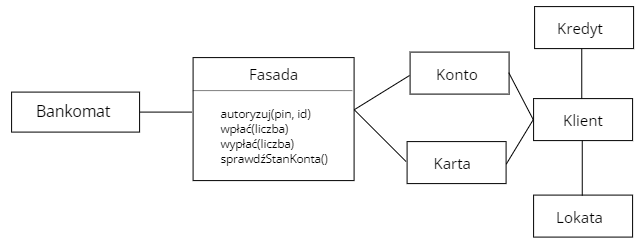
\includegraphics[scale=0.45]{facede.png}
    \caption{Przykładowe zastosowanie fasady na bazie bankomatu.}
  \end{center}
\end{figure}
\newpage

\section{Format pliku z grafem}\label{sec:format-pliku-z-grafem}
Program do wczytywania przyjmuje plik o określonych
właściwościach:
\begin{itemize}
  \item W pierwszym wierszu pliku znajduje się informacja o liczbie wierszy i
        kolumn jakie składają się na graf,
  \item W każdym następnym wierszu znajduję się informacja o tym z jakimi
        innymi wierzchołkami połączony jest dany wierzchołek oraz waga jaka odpowiada
        temu połączeniu.
\end{itemize}
Ze względu na numerowanie wierzchołków od zera, numer wiersza odpowiada
numerowi wierzchołka zwiększonego o jeden.
Przykładowa zawartość pliku:
\lstinputlisting{listings/format.txt}

\section{Uruchomienie Programu}\label{sec:uruchomienie-programu}

\section{Struktura Programu}\label{sec:struktura-programu}
W tym rozdziale przedstawiamy strukturę katalogów naszego programu oraz diagram
klas.

\subsection{Struktura folderów}\label{subsec:struktura-folderów}
Struktura różni się lekko od tej zaprezentowanej w specyfikacjach z racji
przeniesienia projektu na osobną stronę
z system kontroli wersji. Wszystkie nazwy zostały zmienione na język angielski.

\begin{forest}
  for tree={
  font=\ttfamily,
  grow'=0,
  child anchor=west,
  parent anchor=south,
  anchor=west,
  calign=first,
  inner xsep=7pt,
  edge path={
      \noexpand\path [draw, \forestoption{edge}]
      (!u.south west) +(7.5pt,0) |- (.child anchor) pic {folder}
      \forestoption{edge label};
    },
  before typesetting nodes={
      if n=1
        {insert before={[,phantom]}}
        {}
    },
  fit=band,
  before computing xy={l=15pt},
  }
  [\texttt{Grapher}
  [\texttt{documentacy}
    [\texttt{Functional Datasheet}
      [\texttt{images}]
      [\texttt{listings}]
    ]
    [\texttt{Implementational Datasheet}
      [\texttt{images}]
      [\texttt{listings}]
    ]
    [\texttt{Report}
      [\texttt{images}]
      [\texttt{listing}]
    ]
  ]
  [\texttt{src}
    [\texttt{java}
      [\texttt{main}
        [\texttt{java}
          [\texttt{pl.edu.pw.ee.grapher}
            [\texttt{bfs}]
            [\texttt{dijkstra}]
            [\texttt{generator}]
            [\texttt{graph}]
            [\texttt{graphio}]
            [\texttt{utils}]
          ]
        ]
        [\texttt{resources}
          [\texttt{fxml}]
          [\texttt{img}]
          [\texttt{css}]
        ]
      ]
    ]
    [\texttt{test}
      [\texttt{java}
        [\texttt{pl.edu.pw.ee.grapher}
          [\texttt{<te same foldery co w src/java>}]
          [\texttt{testData}]
        ]
      ]
      [\texttt{resources}]
    ]
  ]
  ]
\end{forest}

\subsection{Diagram Klas}\label{subsec:diagram-klas}
Nowy diagram klas został umieszczony w pliku HTML w folderze \textit{diagram} ze względu na jego
rozbudowaną strukturę.
\begin{figure}[h]
  \begin{center}
    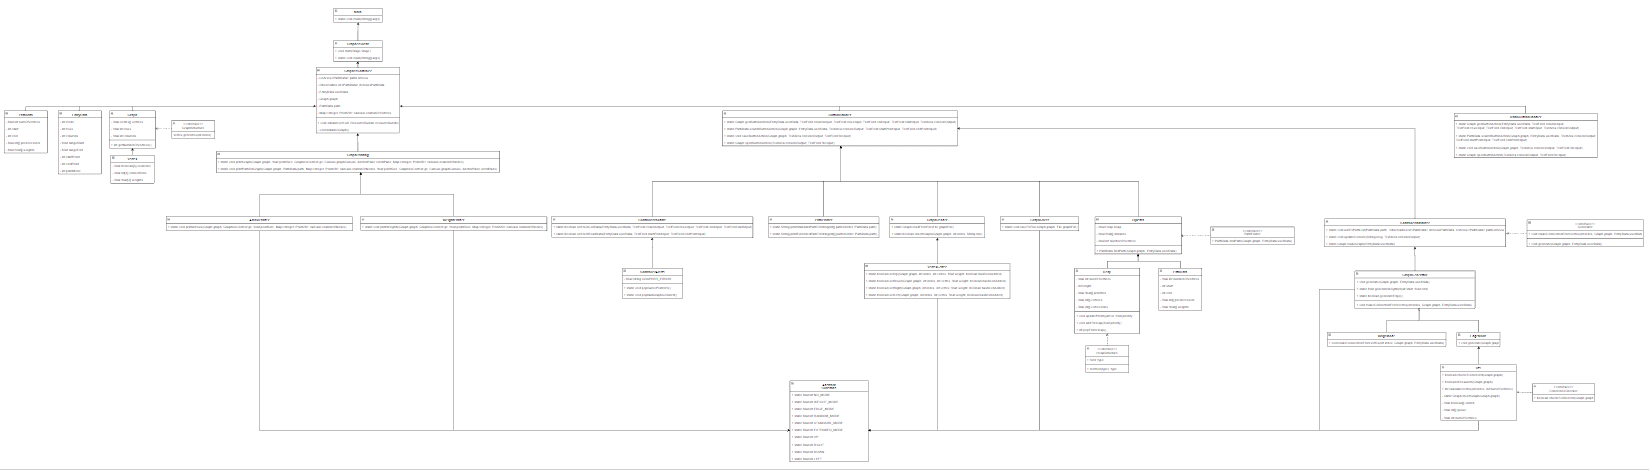
\includegraphics[scale=0.33]{diagram.png}
    \caption{Diagram klas.}
  \end{center}
\end{figure}

\section{Wykorzystane algorytmy}\label{sec:wykorzystane-algorytmy}
Nasz program wykorzystuje dwa algorytmy, które opisujemy w poniższych
podrozdziałach.

\subsection{Algorytm Dijkstry}\label{subsec:algorytm-dijkstry}
Algorytm Dijkstry liczy najkrótszą odległość od wierzchołka początkowego do
wszystkich innych wierzchołków,
ale w naszej implementacji skupiamy się jedynie na najkrótszej ścieżce między
wierzchołkami zadanymi przez
użytkownika. Algorytm ten korzysta z kopca pełniącego funkcje kolejki
priorytetowej oraz trzech tablic przechowujących
poprzedników, wagi połączeń i całkowity dystans.
Algorytm dodaje odwiedzane wierzchołki do kolejki priorytetowej, a następnie
pobiera je z niej aktualizując dystans,
dopóki kopiec nie jest pusty. Następnie zaczynając od wierzchołka końcowego
(podanego przez użytkownika) cofamy się aż trafimy do wierzchołka początkowego.
Podczas cofania zapisujemy przez jakie wierzchołki przeszliśmy oraz jaka była
waga takiego przejścia.
\begin{figure}[h]
  \begin{center}
    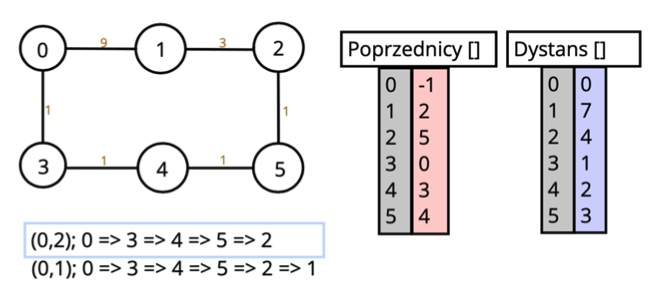
\includegraphics[scale=0.5]{dijkstra.png}
    \caption{Przykładowe działanie algorytmu Dijksty.}
  \end{center}
\end{figure}
\newpage

\subsection{Breadth-first search(BFS)}\label{subsec:breadth-first-search(bfs)}
Nasz program wykorzystuje do sprawdzania spójności algorytm BFS. Nasza
implementacja różni się od pierwotnie zakładanej w specyfikacji
implementacyjnej
projektu, ponieważ wykorzystaliśmy algorytm \textit{Kosaraju}, który wjaśnimy
niżej.
Algorytm w celu sprawdzenia spójności tworzy tablicę poprzedników o długości
odpowiadającej ilości wierzchołków
oraz zapełnia ją wartościami -1. Rozpoczynając iteracje od wierzchołka zero aż
do ostatniego wierzchołka.
Algorytm BFS polega na sprawdzeniu spójności przez przechodzenie po sąsiadach
danego wierzchołka i jeżeli algorytmowi uda się
przejść po wszystkich wierzchołkach(oczywiście jeżeli algorytm zostanie
wykonany ze wszystkich wierzchołków co gwarantuje tak zwaną \textit{silną
  spójność}), czyli w tablicy odwiedzonych wierzchołków wszystkie mają wartość
\texttt{true}, to znaczy, że graf jest spójny.
\begin{figure}[h]
  \begin{center}
    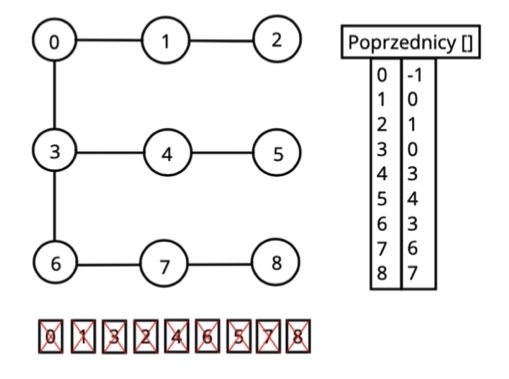
\includegraphics[scale=0.5]{bfs.png}
    \caption{Przykładowe działanie algorytmu BFS.}
  \end{center}
\end{figure}
\newpage

\subsection{Strongly Connected Components (Algorytm Kosaraju)}\label{subsec:kosaraju}
Algorytm Kosaraju polega na wykorzystaniu silnych związków pomiędzy
wierzchołkami grafu. Pierwszym krokiem jest włączenie BFS'a z zerowego
wierzchołka i sprawdzenie, czy graf jest spójny.
Jeżeli jest spójny to trzeba odwrócić graf, to znaczy zamienić zwroty
wszystkich krawędzi grafu żeby biegły w przeciwną stronę, a następnie
uruchamiamy BFS'a po raz drugi ale już na odwróconym grafie.
Spójność po drugim uruchomieniu sprawdzania za pomocą algorytmu zapewnia nam
spójność całego grafu.

\newpage

\section{Wywołania programu}\label{sec:wywołania-programu}
W poniższym rozdziale zostaną pokazane dwa przykładowe wywołania programu, w
trybie WageMode, a także EdgeMode.
Zaprezentowana zostanie generacja, szukanie najkrótszej ścieżki między dwoma
zadanymi punktami,
a także widok listy pozwalający na szybkie przełączenie się między wcześniej
wyznaczonymi ścieżkami.

\begin{figure}[h]
  \begin{center}
    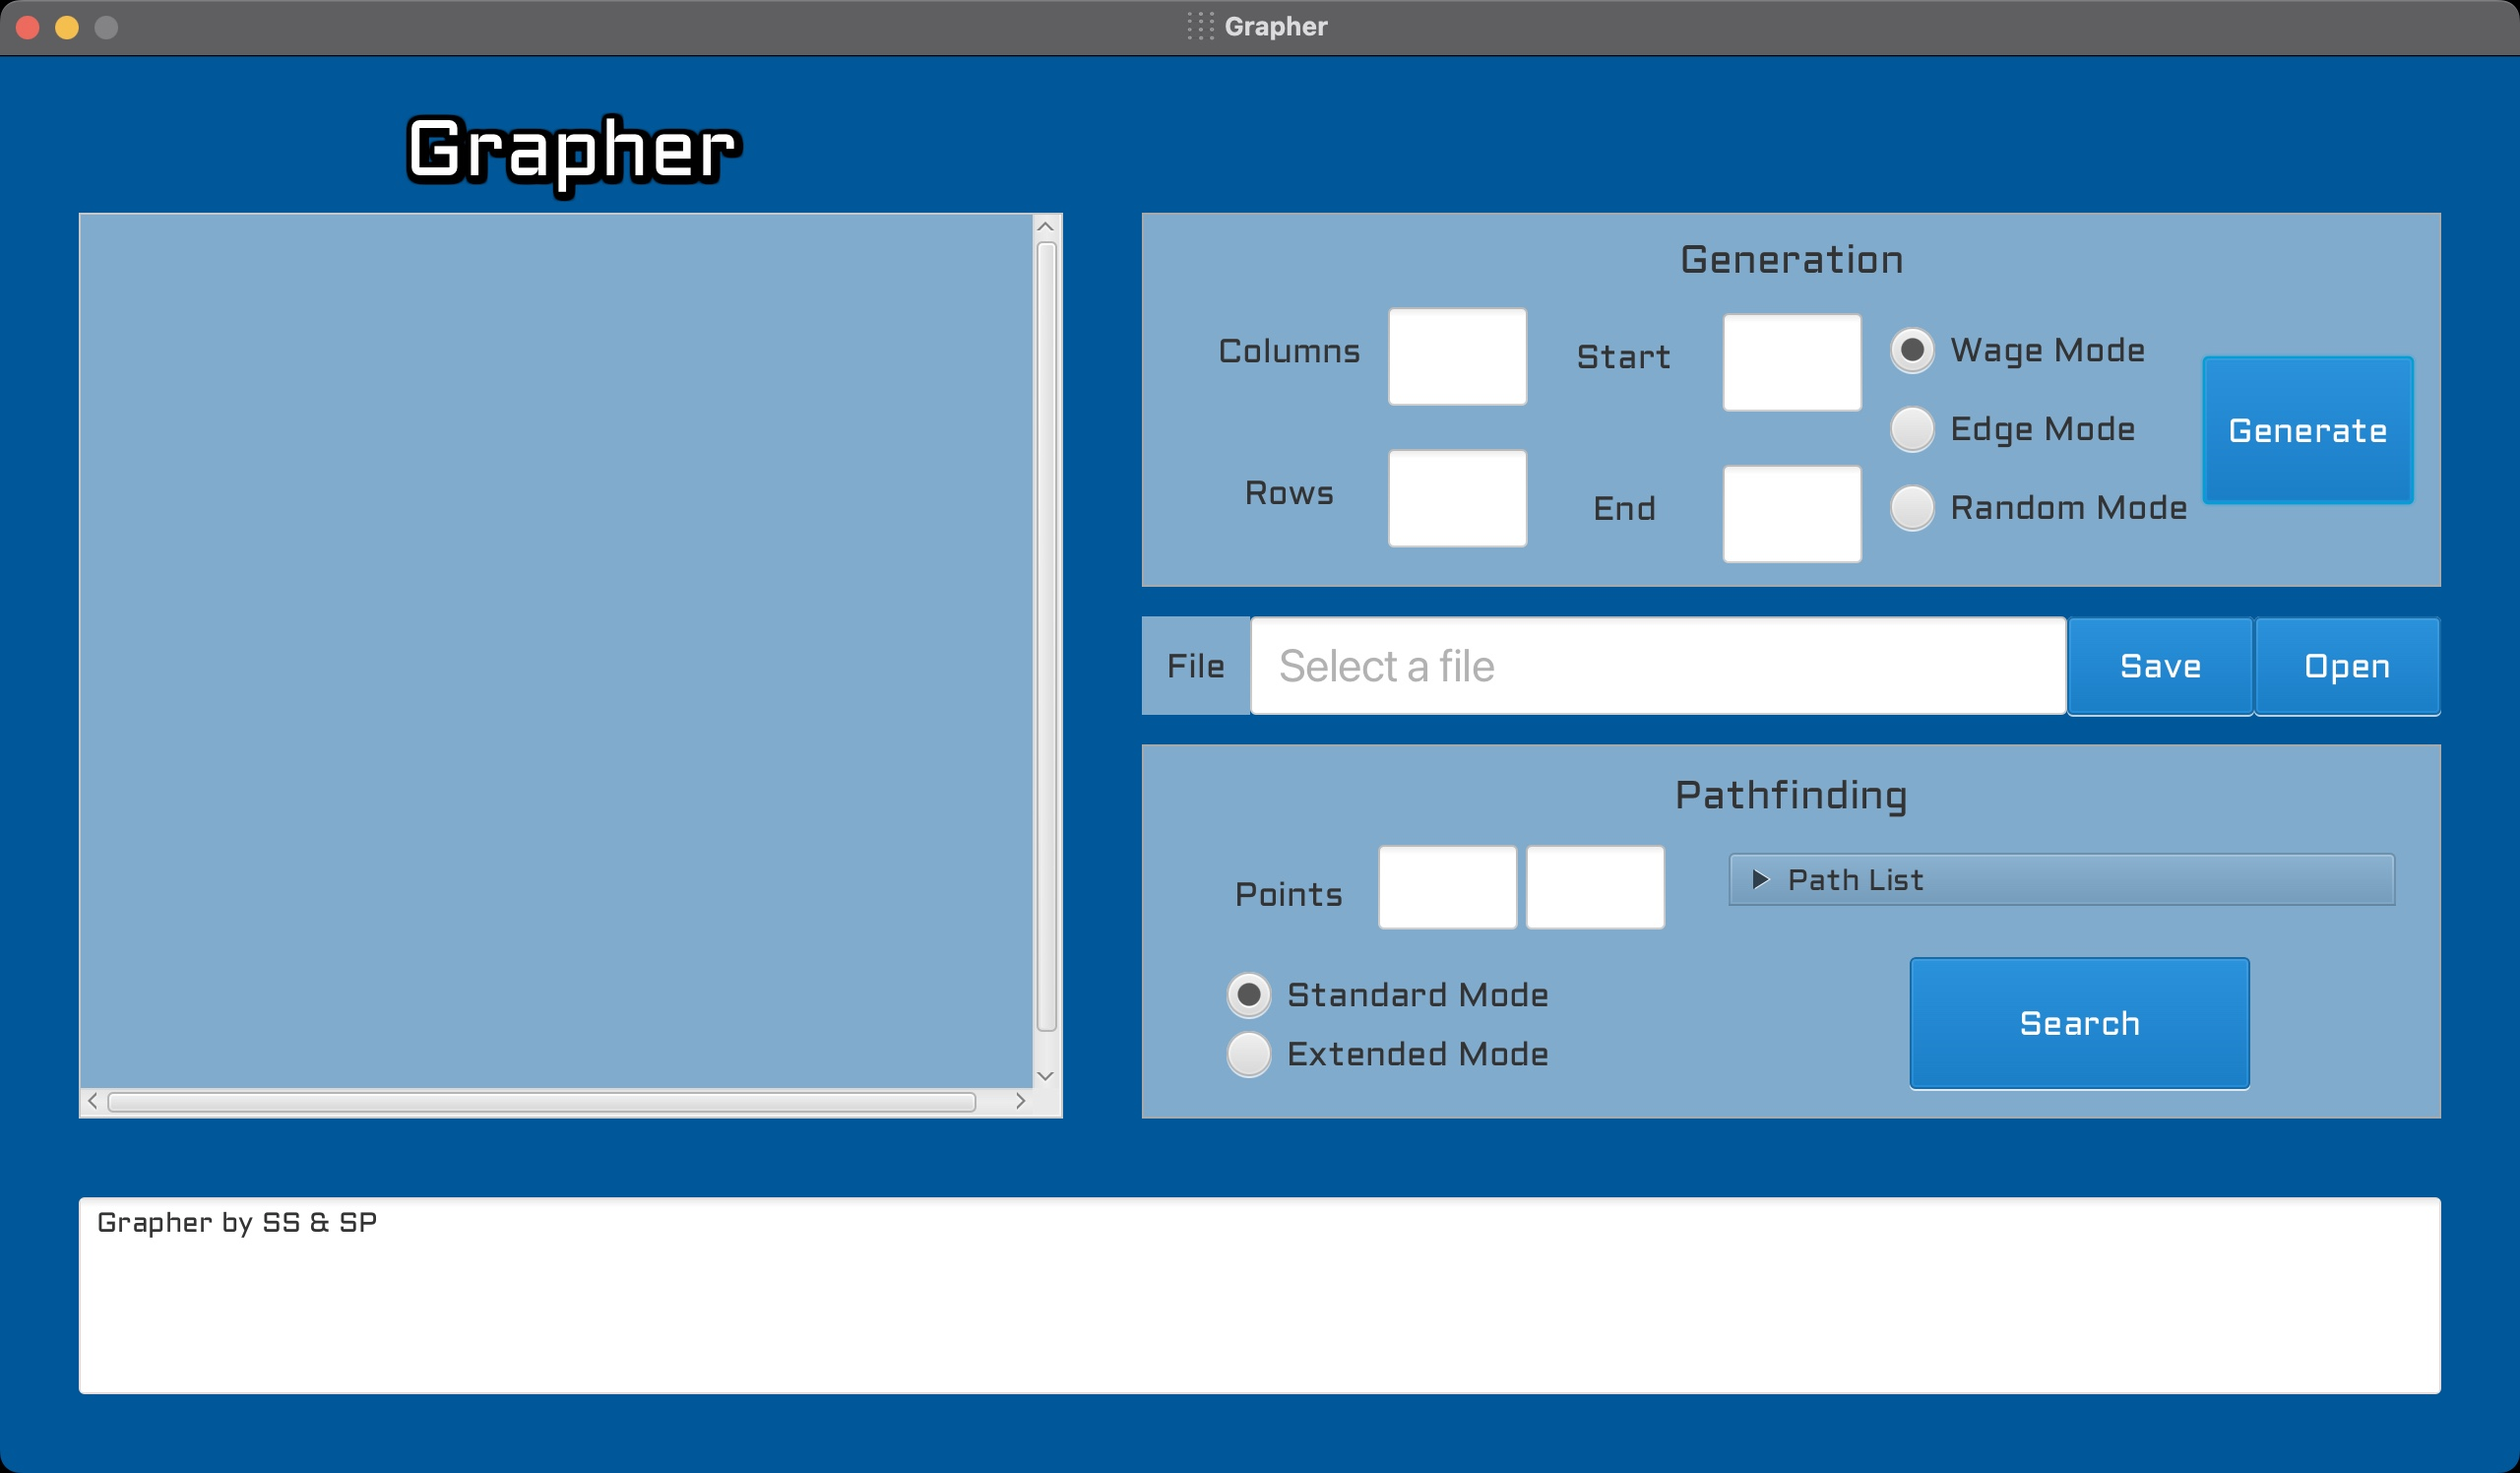
\includegraphics[scale=0.165]{graperStartScreen.jpg}
    \caption{Ekran startowy aplikacji witający użytkownika.}
  \end{center}
\end{figure}

Użytkownik po uruchomieniu aplikacji widzi wyżej pokazany ekran. Ekran ten
składa się z pola na rysowanie grafu, okienka z generacją, obsługą pliku oraz
szukaniem ścieżek.
\newpage

\subsection{Tryb WageMode}\label{subsec:wywołania-wagemode}
Poniżej pokażemy jak wygląda działanie trybu Wage Mode w naszej aplikacji.

\begin{figure}[h]
  \begin{center}
    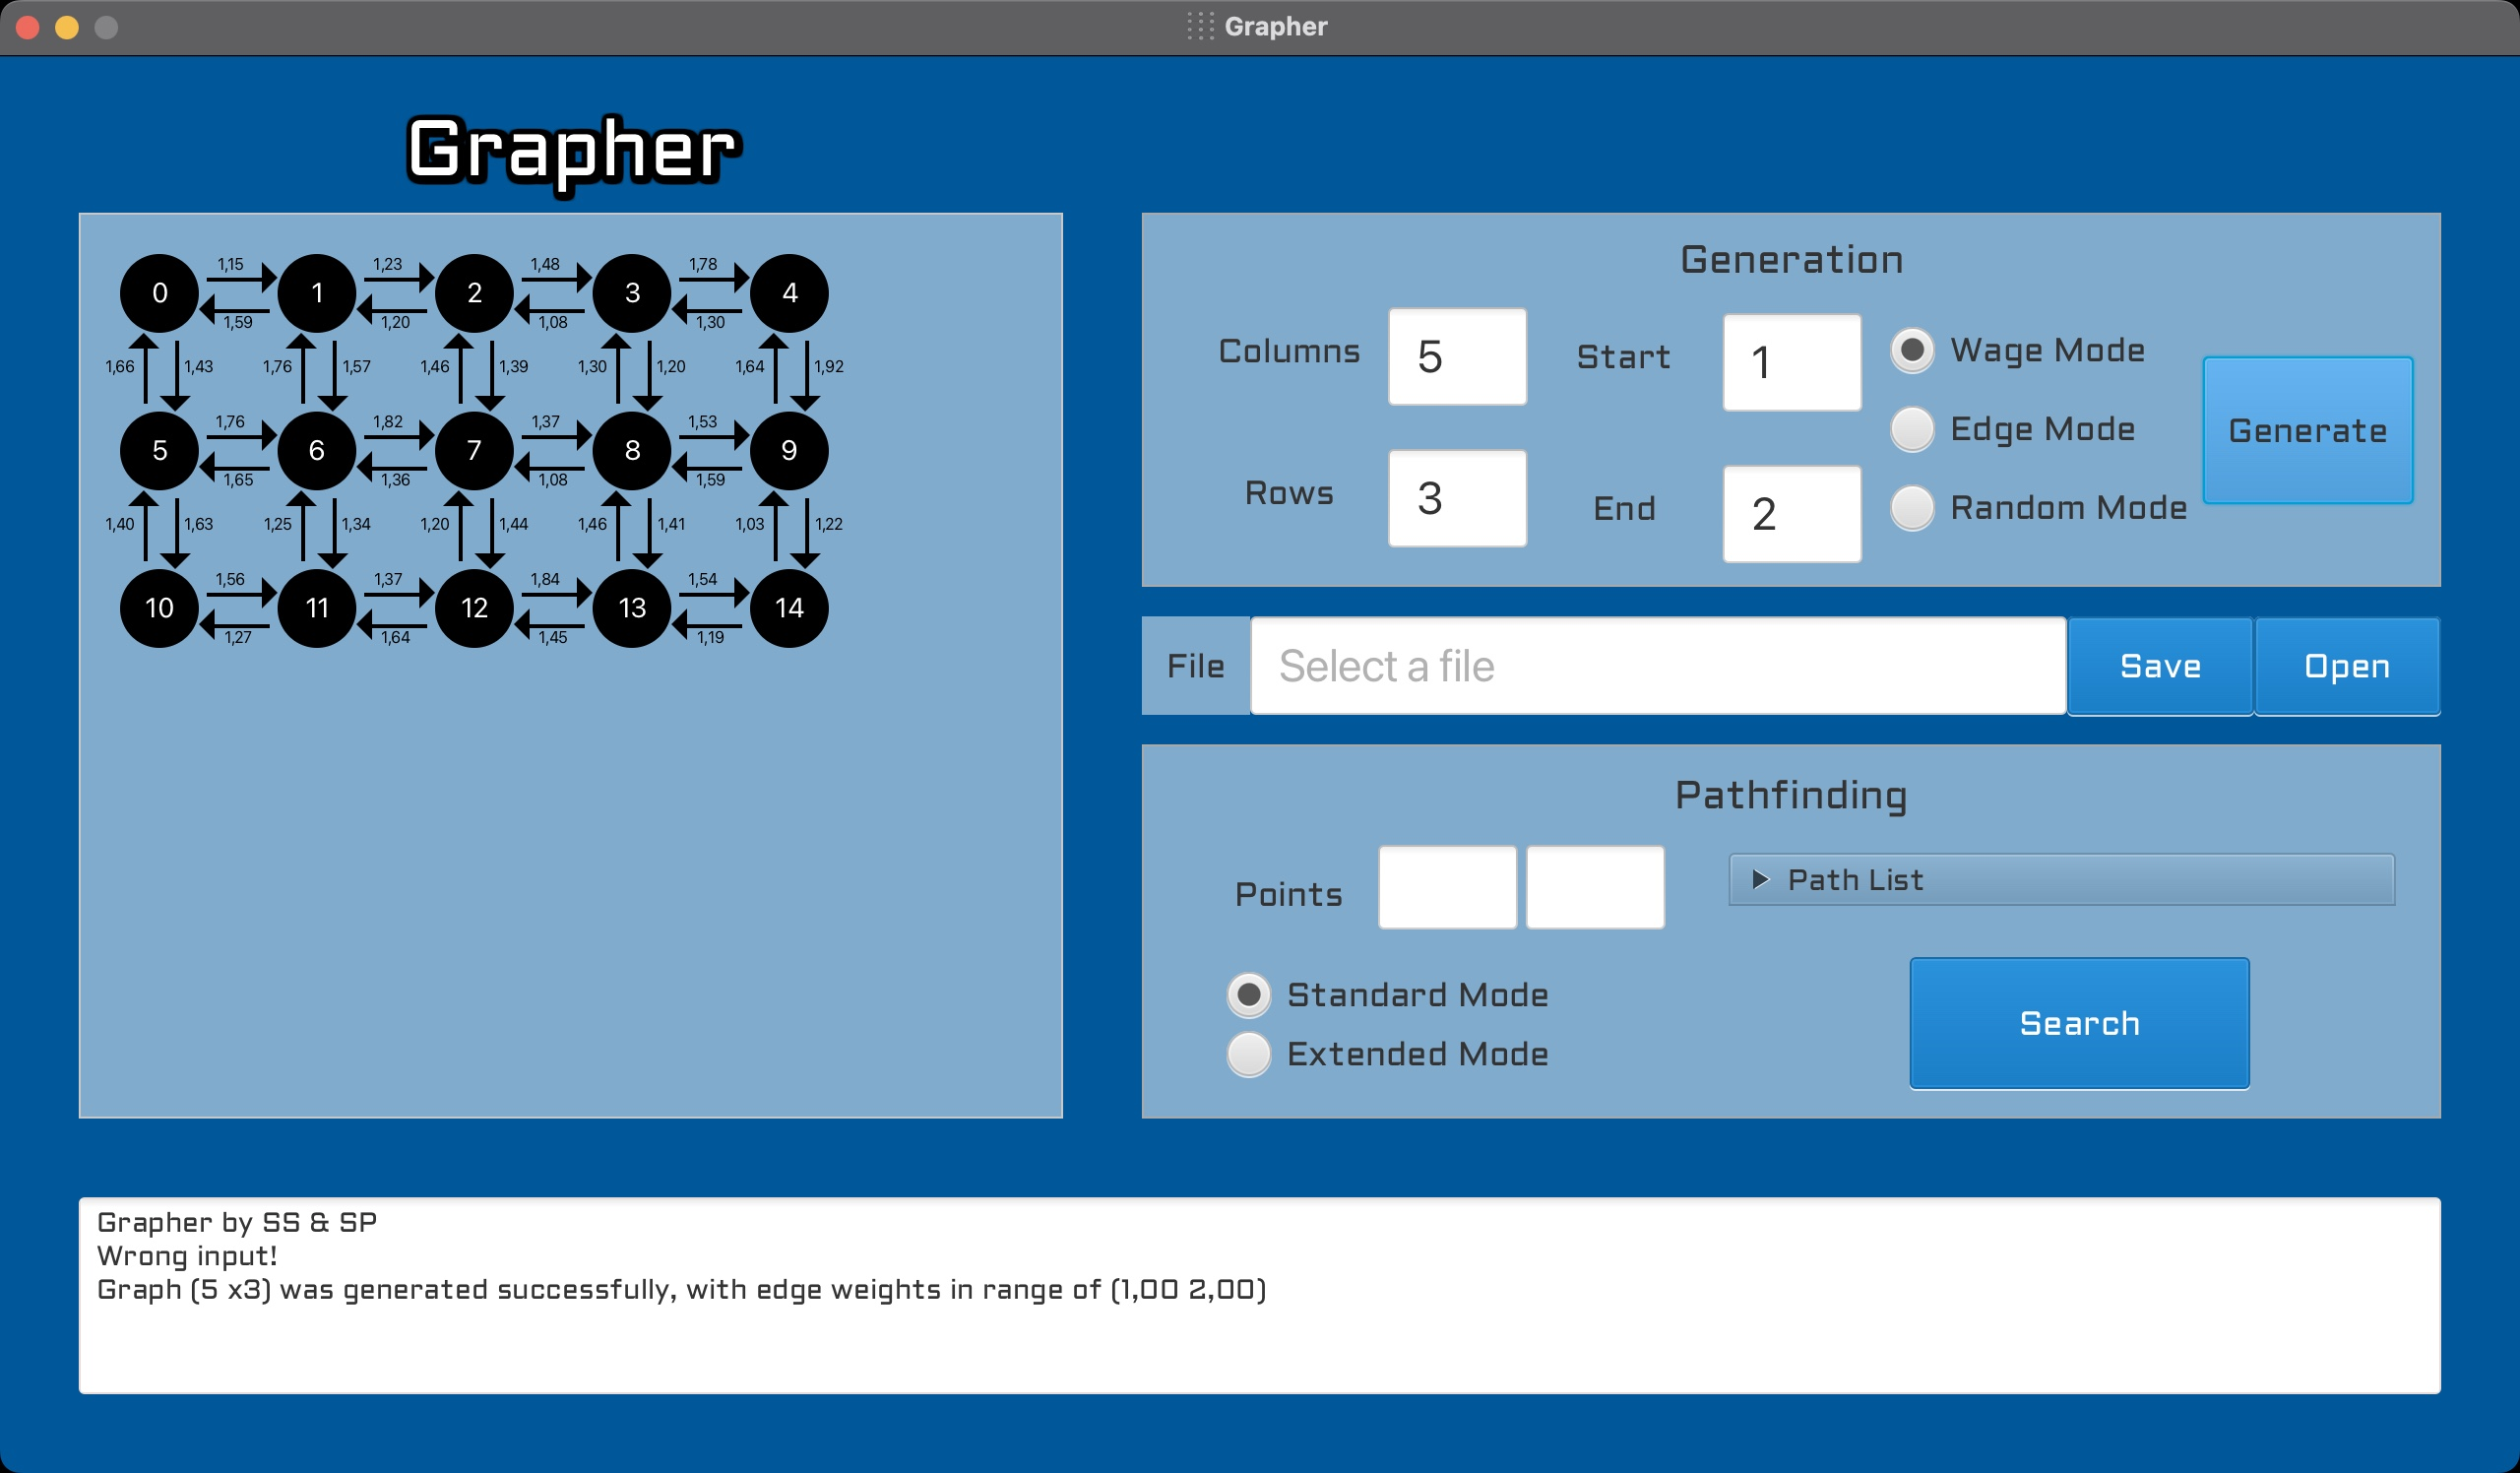
\includegraphics[scale=0.165]{grapherWageModeGeneration.jpg}
    \caption{Przykładowy graf stworzony w trybie WageMode.}
  \end{center}
\end{figure}

Użytkownik zgodnie z wprowadzonymi danymi może wygenerować graf, jeśli graf
posiada poniżej 3600 wierzchołków, graf zostanie wyświetlony po lewej stronie
aplikacji.
\newpage

\begin{figure}[h]
  \begin{center}
    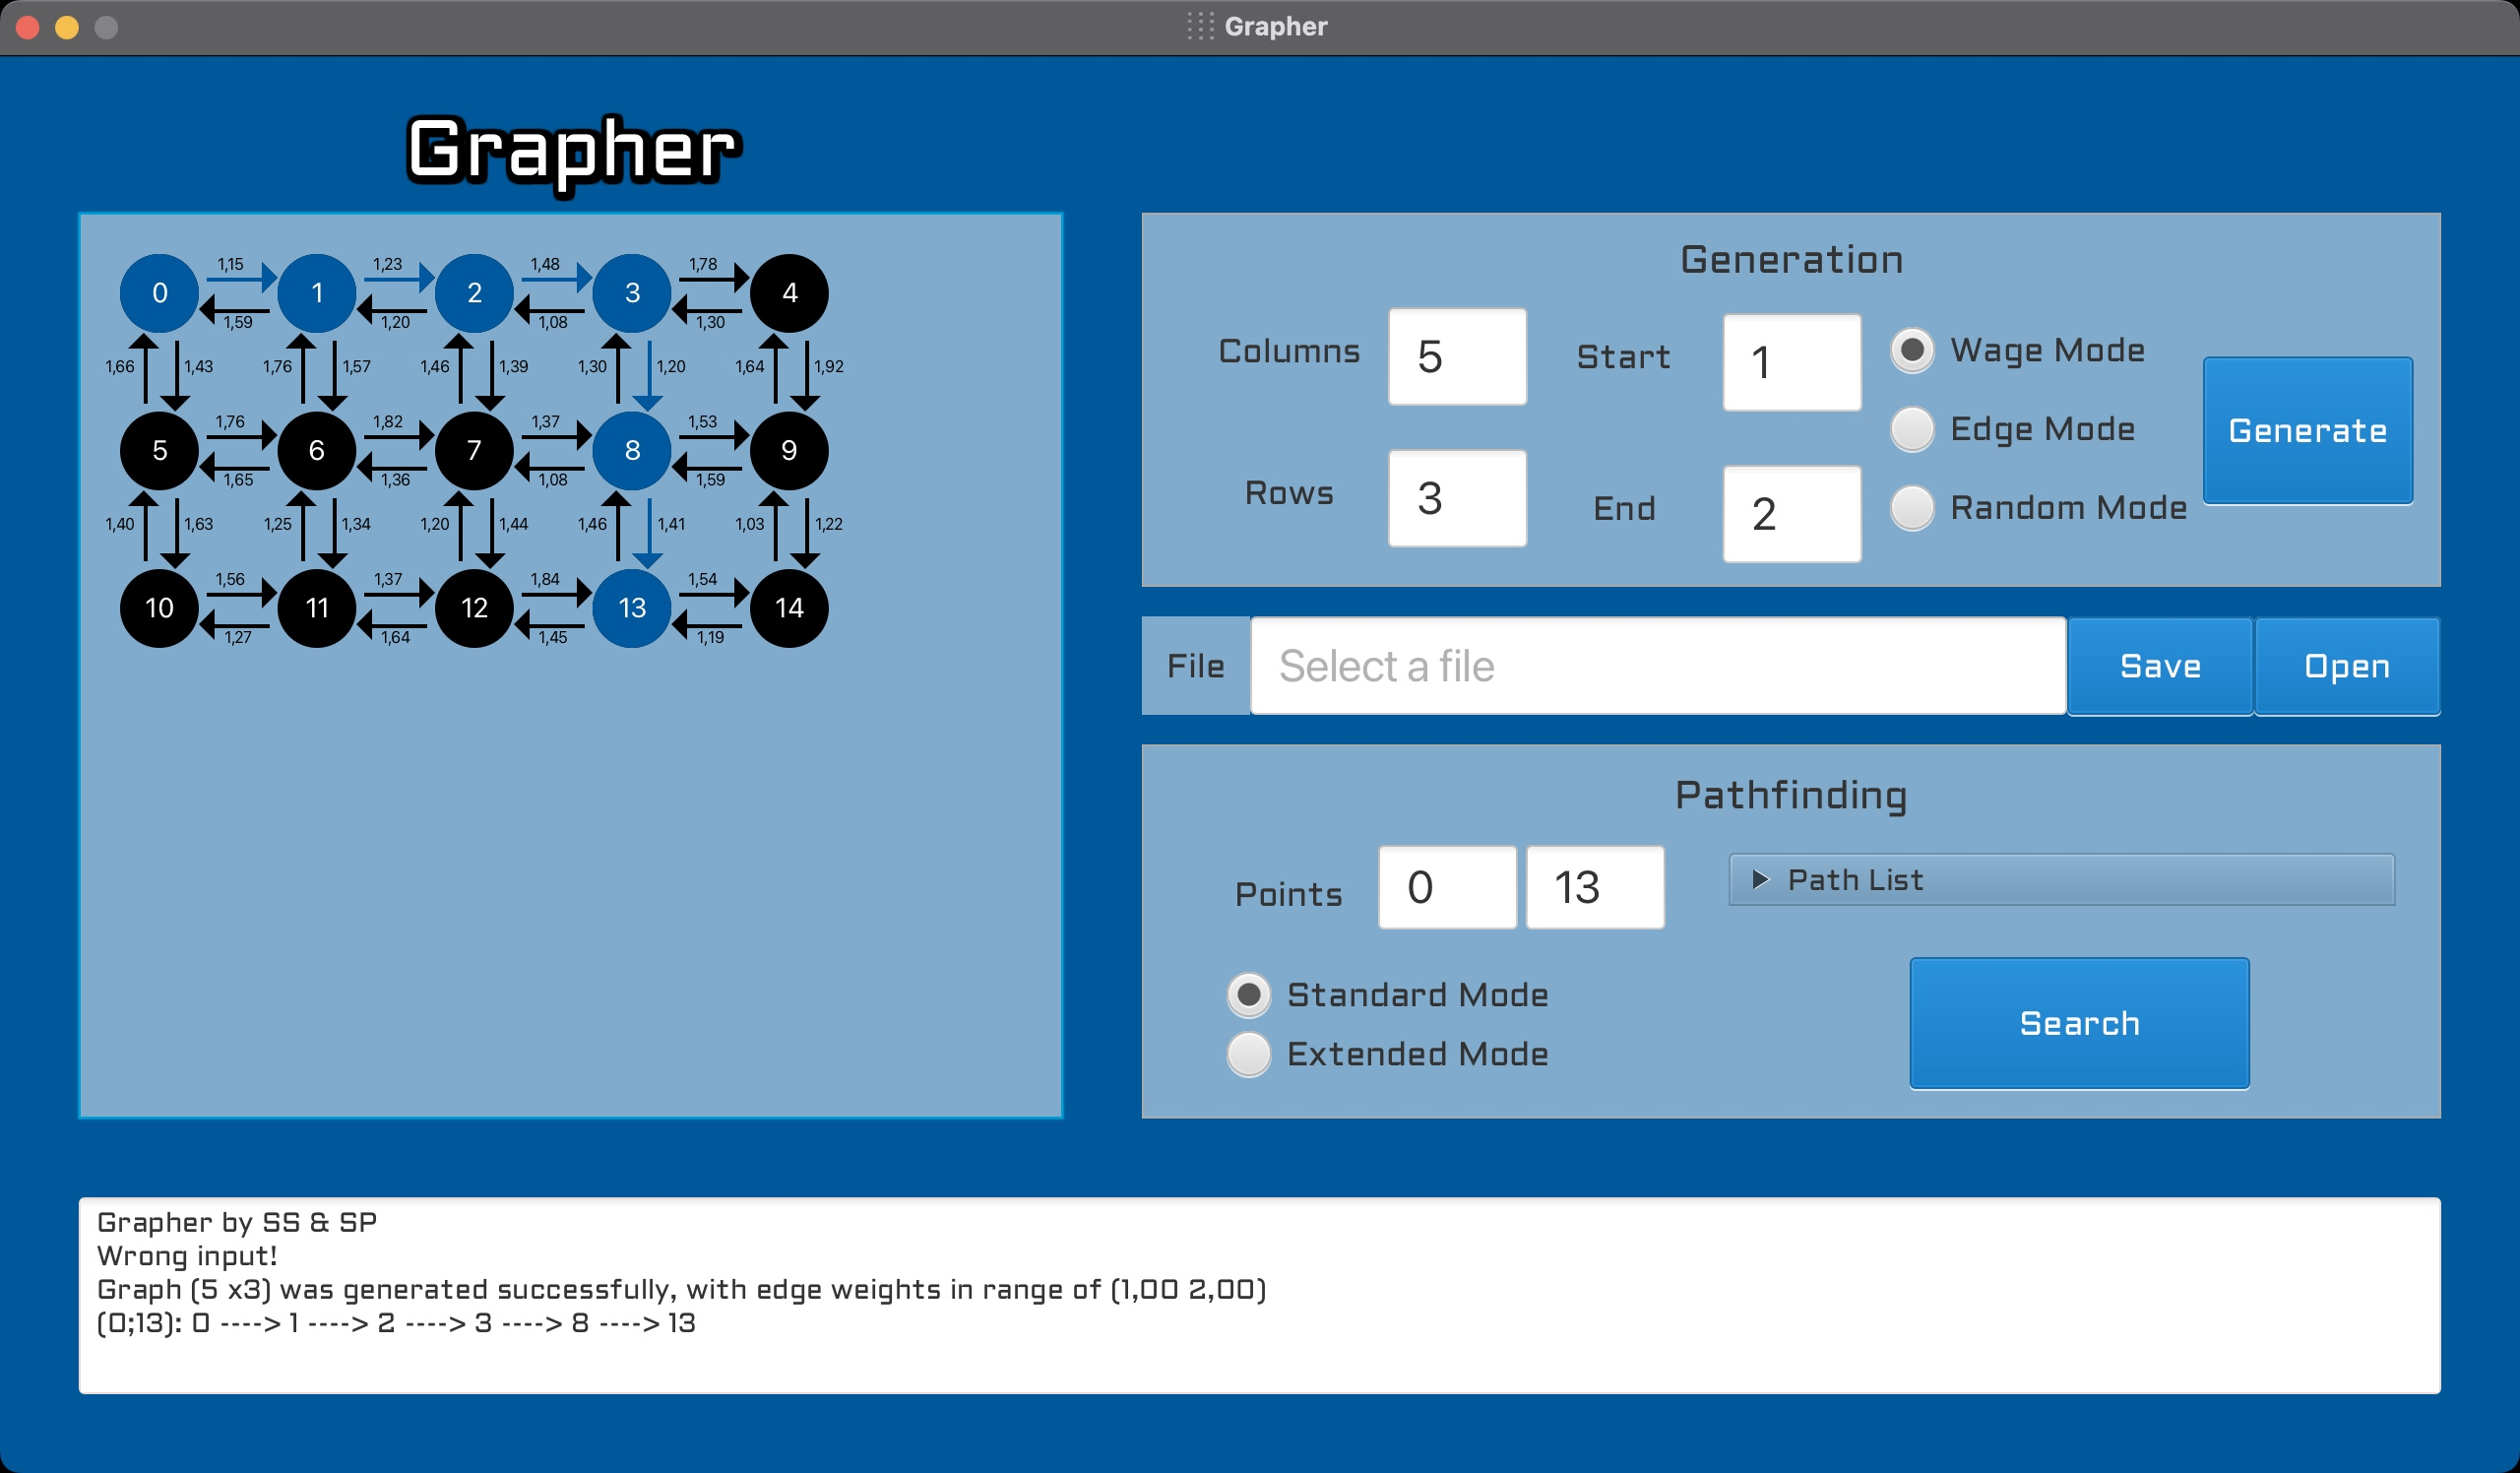
\includegraphics[scale=0.165]{grapherWageModeWithPath.jpg}
    \caption{Ścieżka znaleziona w grafie typu WageMode.}
  \end{center}
\end{figure}

Program umożliwia, też wyszukiwanie ścieżki między zadanymi punktami, co
prezentuje powyższy zrzut ekranu.
\newpage

\begin{figure}[h]
  \begin{center}
    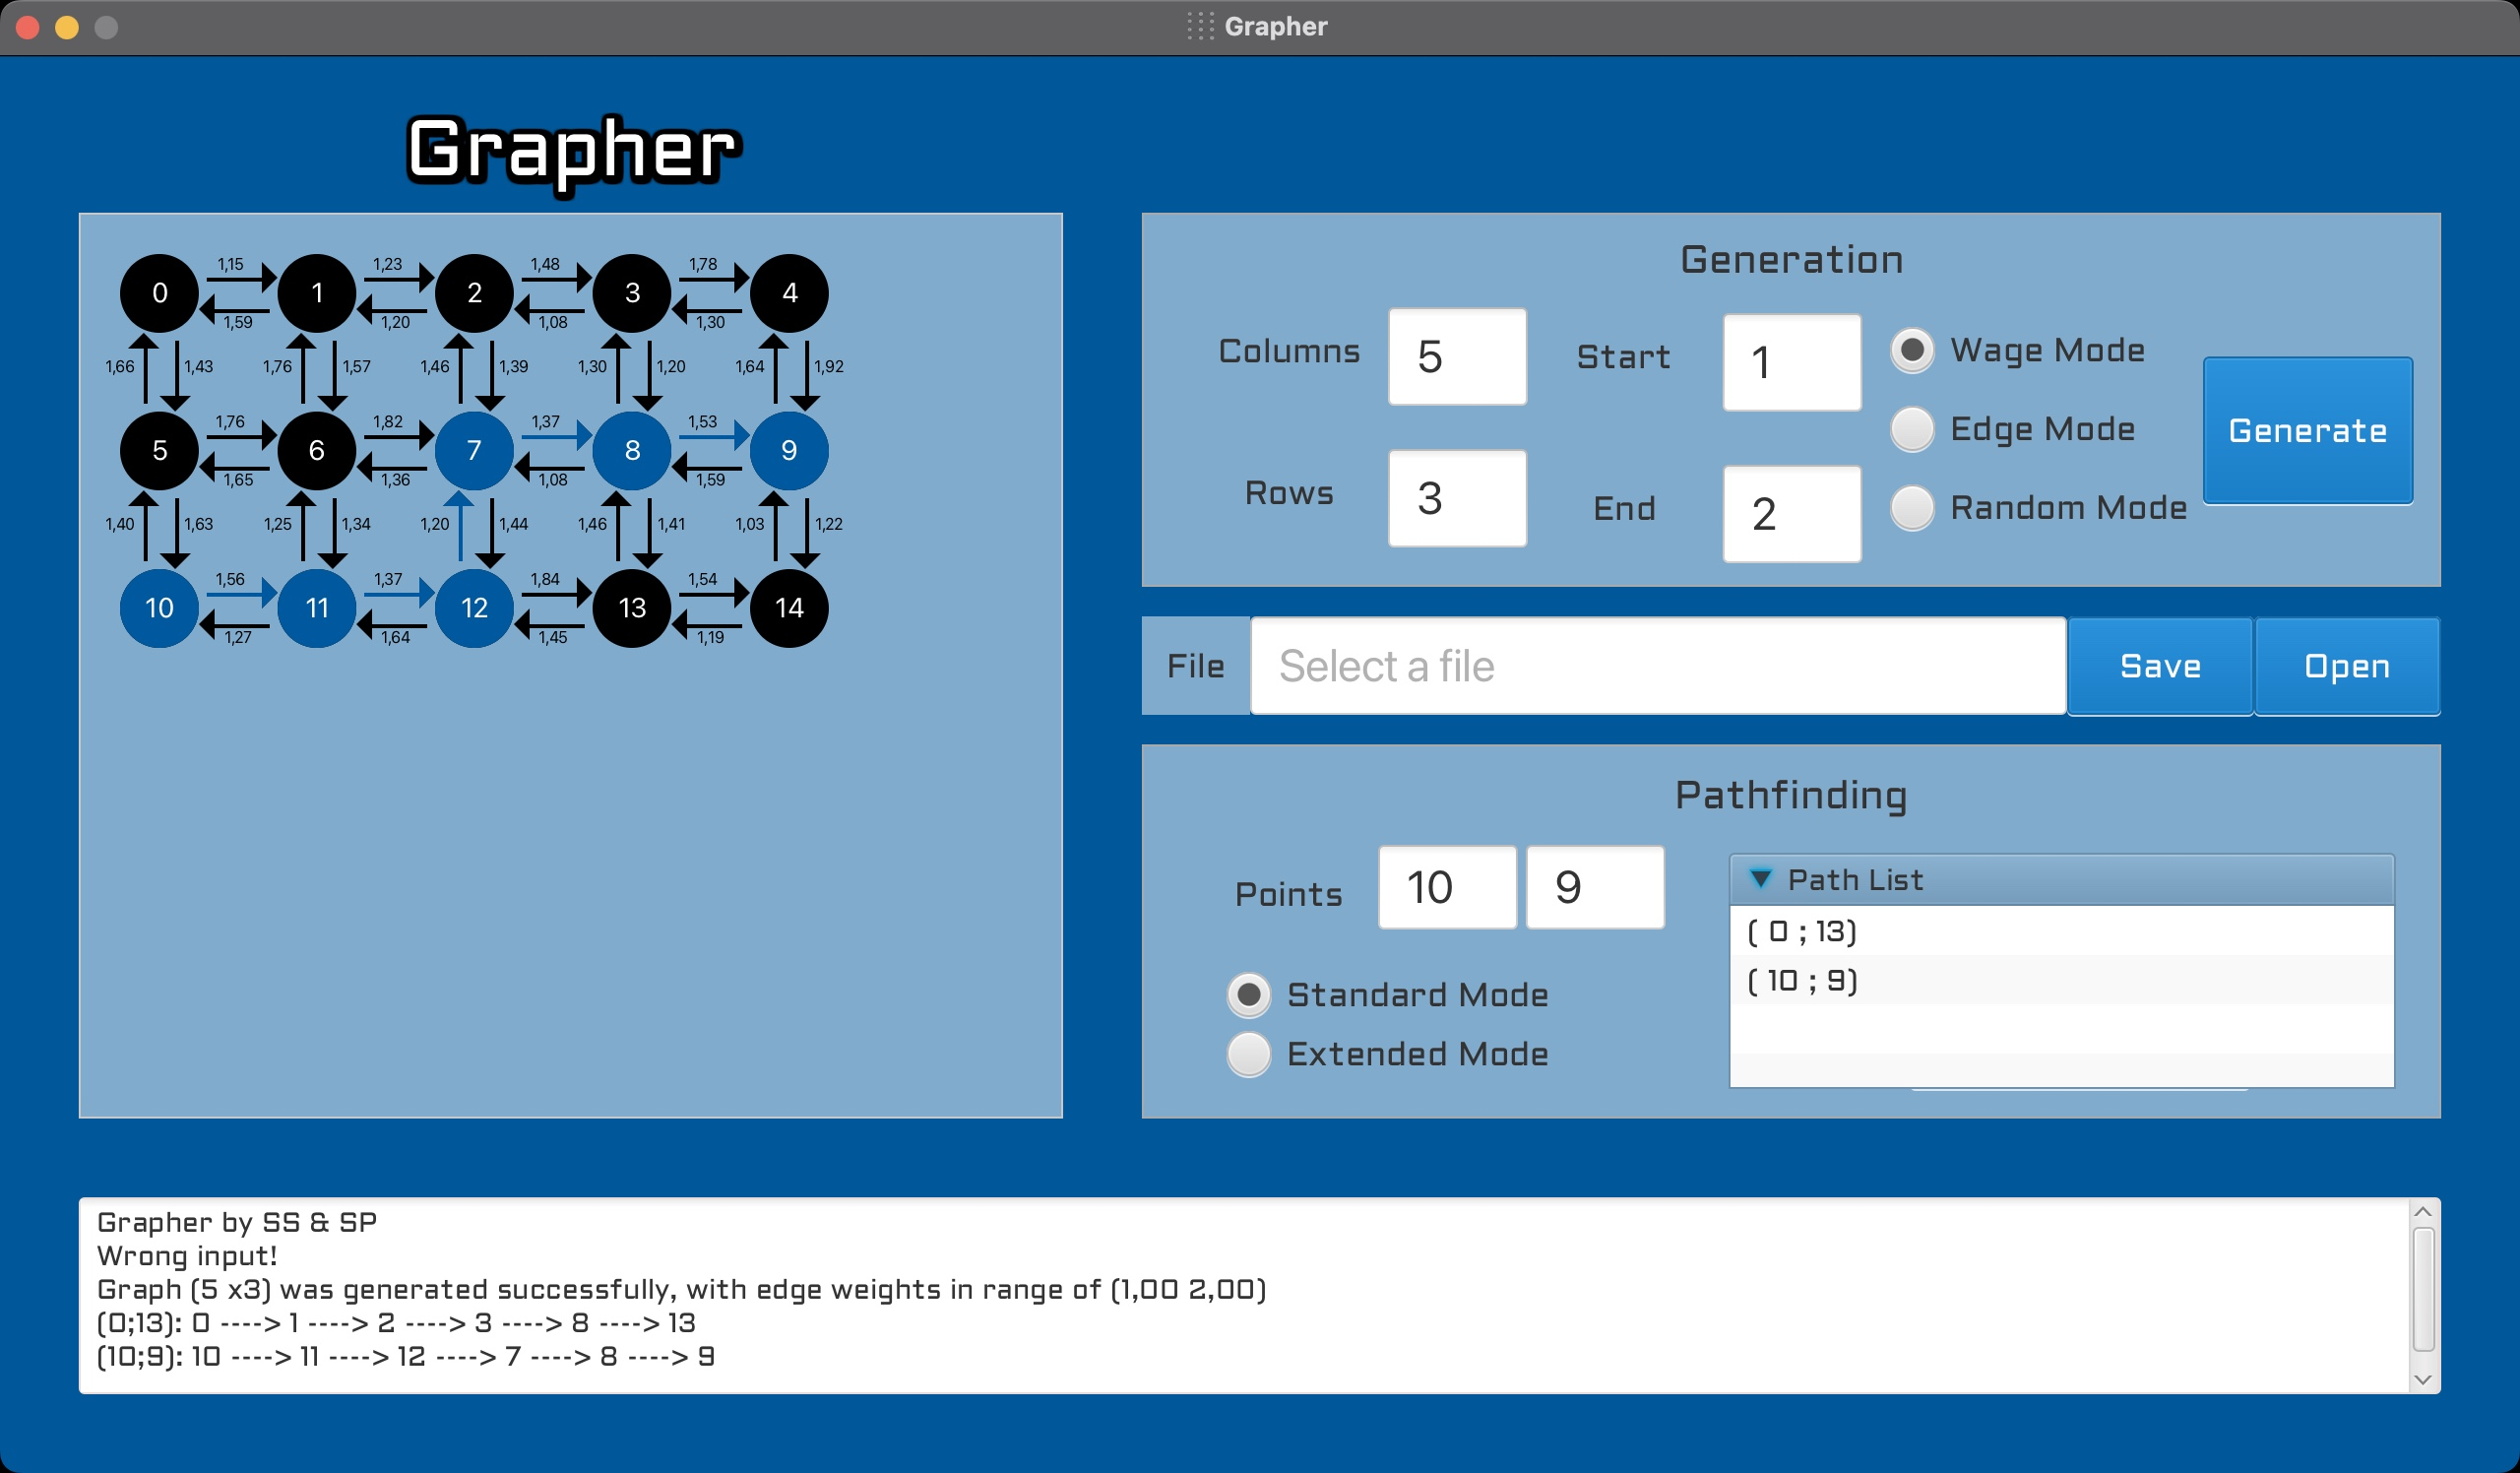
\includegraphics[scale=0.165]{grapherWageModePathList.jpg}
    \caption{Lista poprzednio znalezionych ścieżek w wygenerowanym grafie.}
  \end{center}
\end{figure}

Użytkownik nie traci informacji o znalezionych ścieżkach, wszystkie
dotychczasowo znalezione ścieżki na bieżącym grafie zapisane są w pamięci
aplikacji i dostępne z poziomu listy "Path List".
\newpage

\subsection{Tryb EdgeMode}\label{subsec:wywołania-edgemode}
Tryb Edge Mode był już powyżej prezentowany, a tutaj pokażemy jego użycie.

\begin{figure}[h]
  \begin{center}
    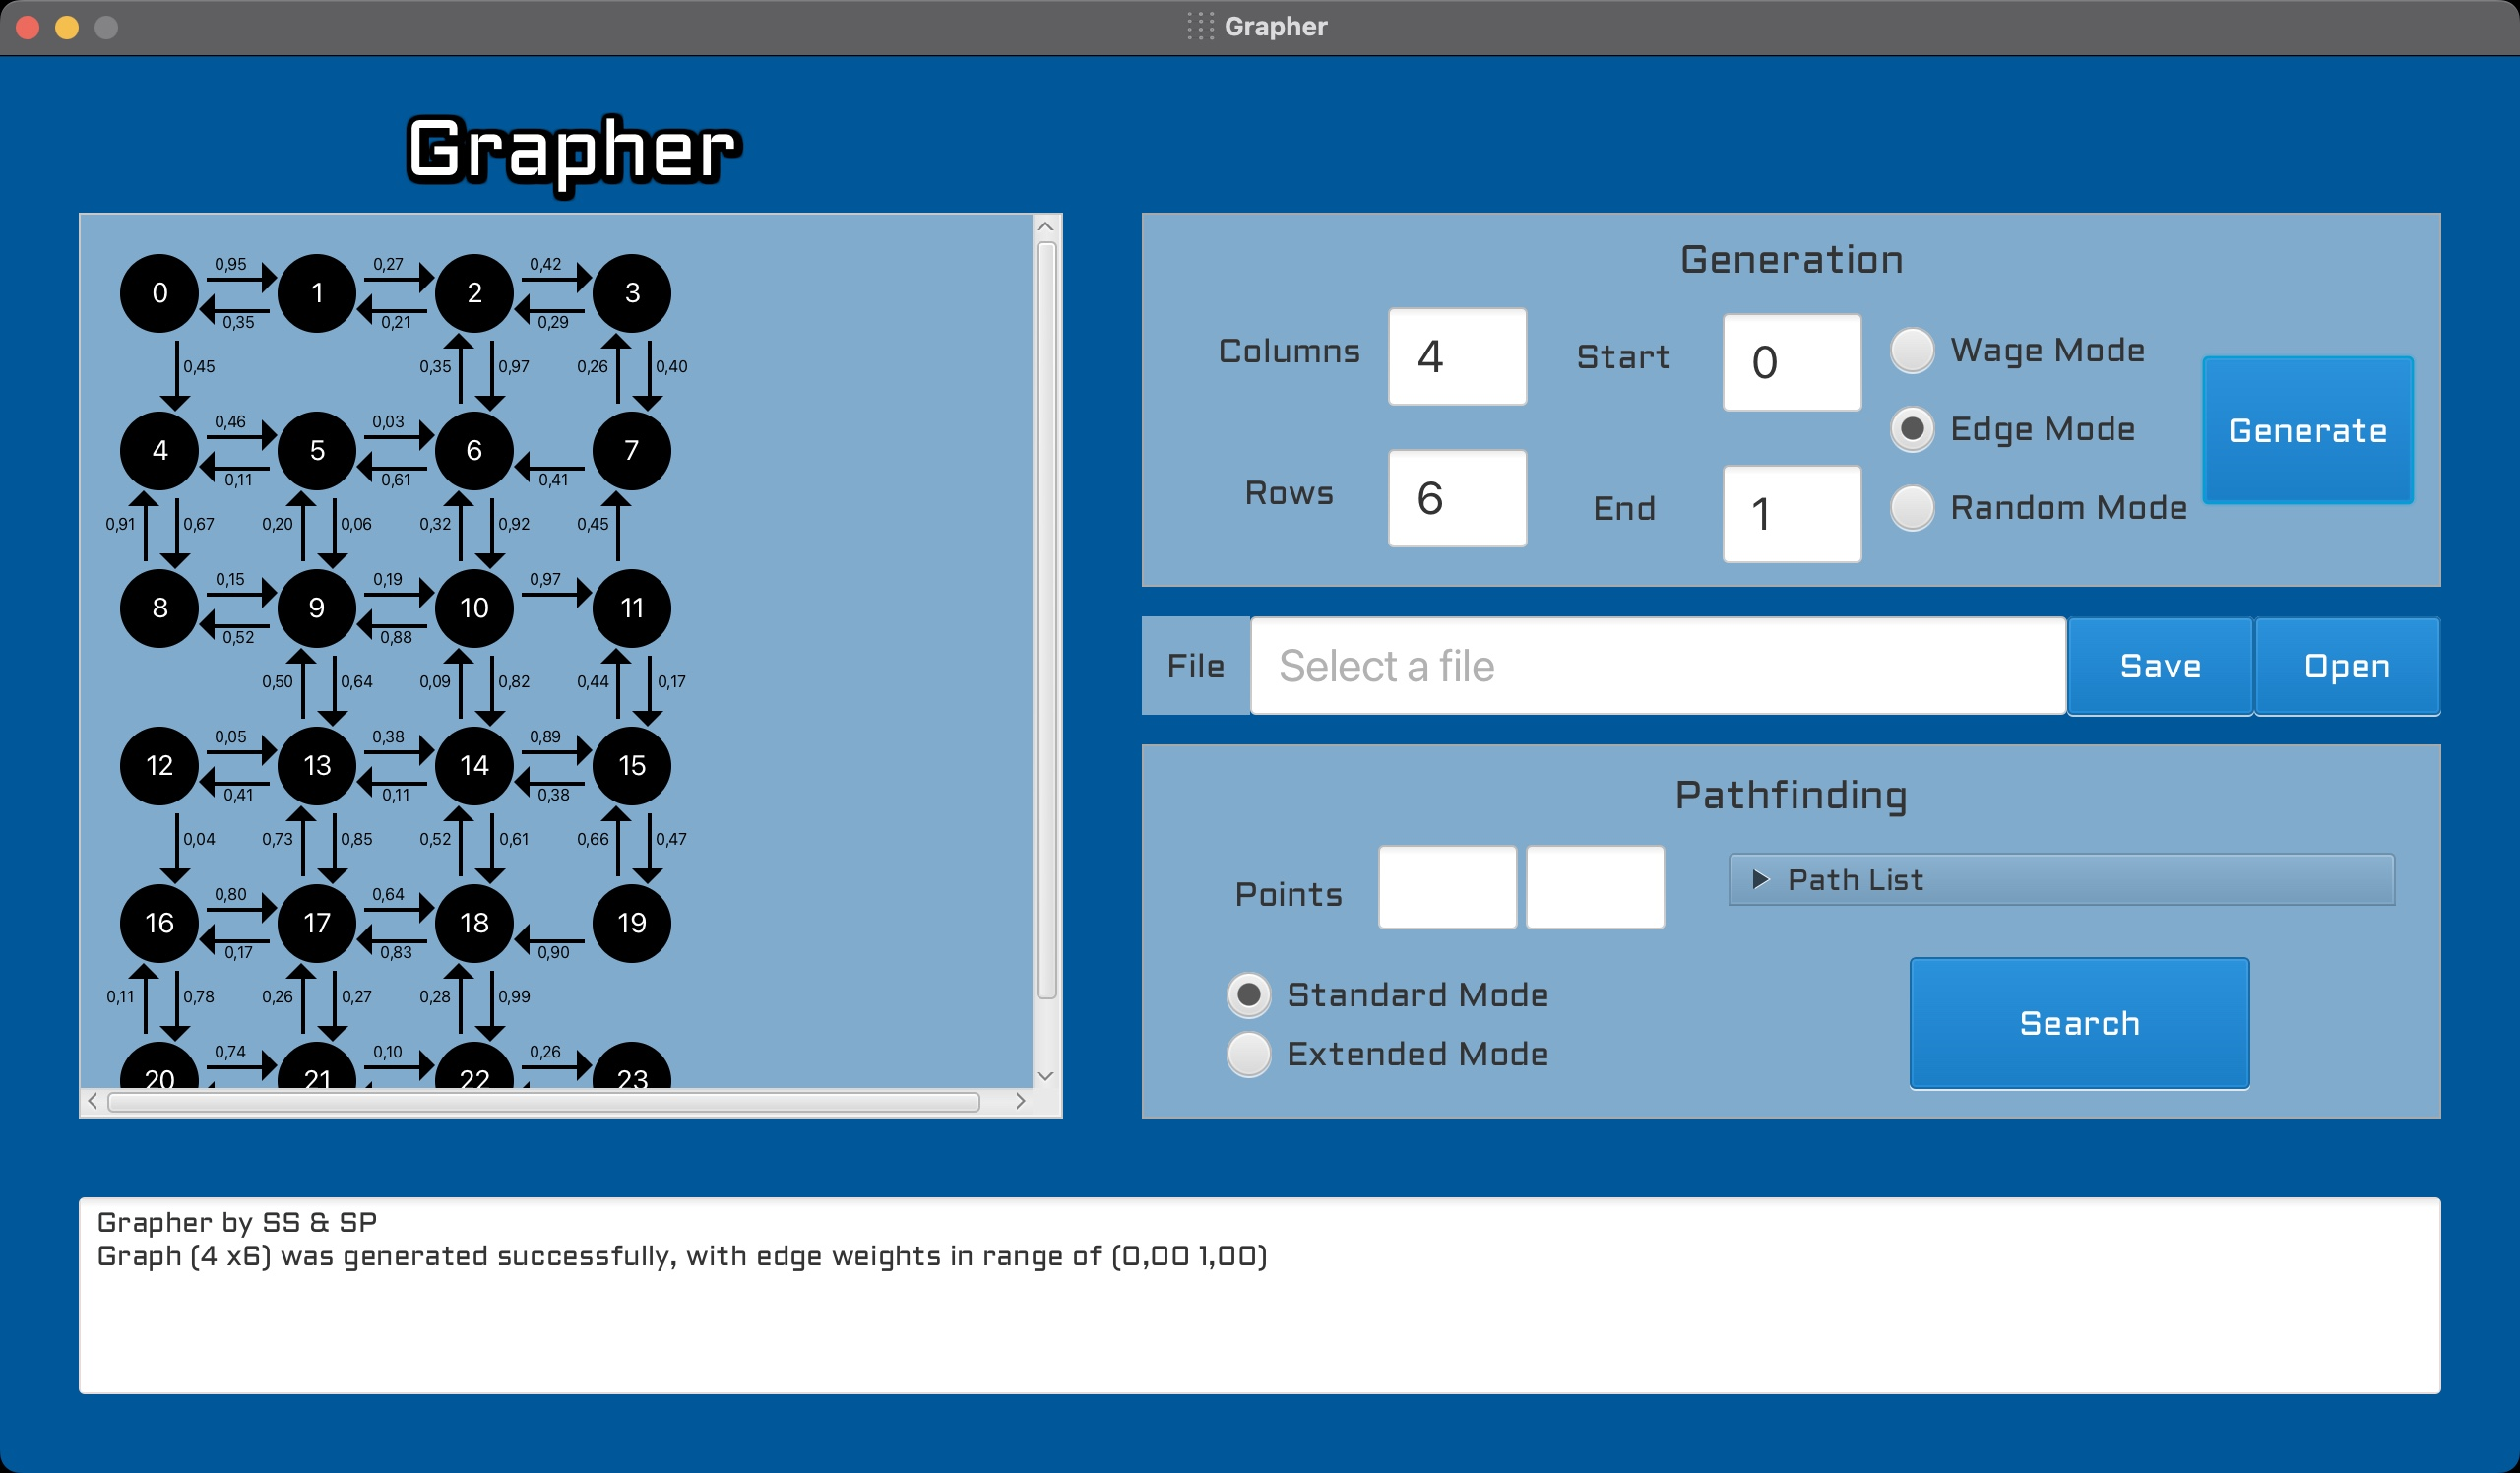
\includegraphics[scale=0.165]{grapherEdgeModeGeneration.jpg}
    \caption{Przykładowy graf spójny wygenerowany w trybie EdgeMode}
  \end{center}
\end{figure}

Podobnie do generacji zgodnie z trybem WageMode użytkownik ma możliwość
generacji i wyświetlania grafu, jeśli wygenerowany graf spełnia wymagania
wyświetlania.
\newpage

\begin{figure}[h]
  \begin{center}
    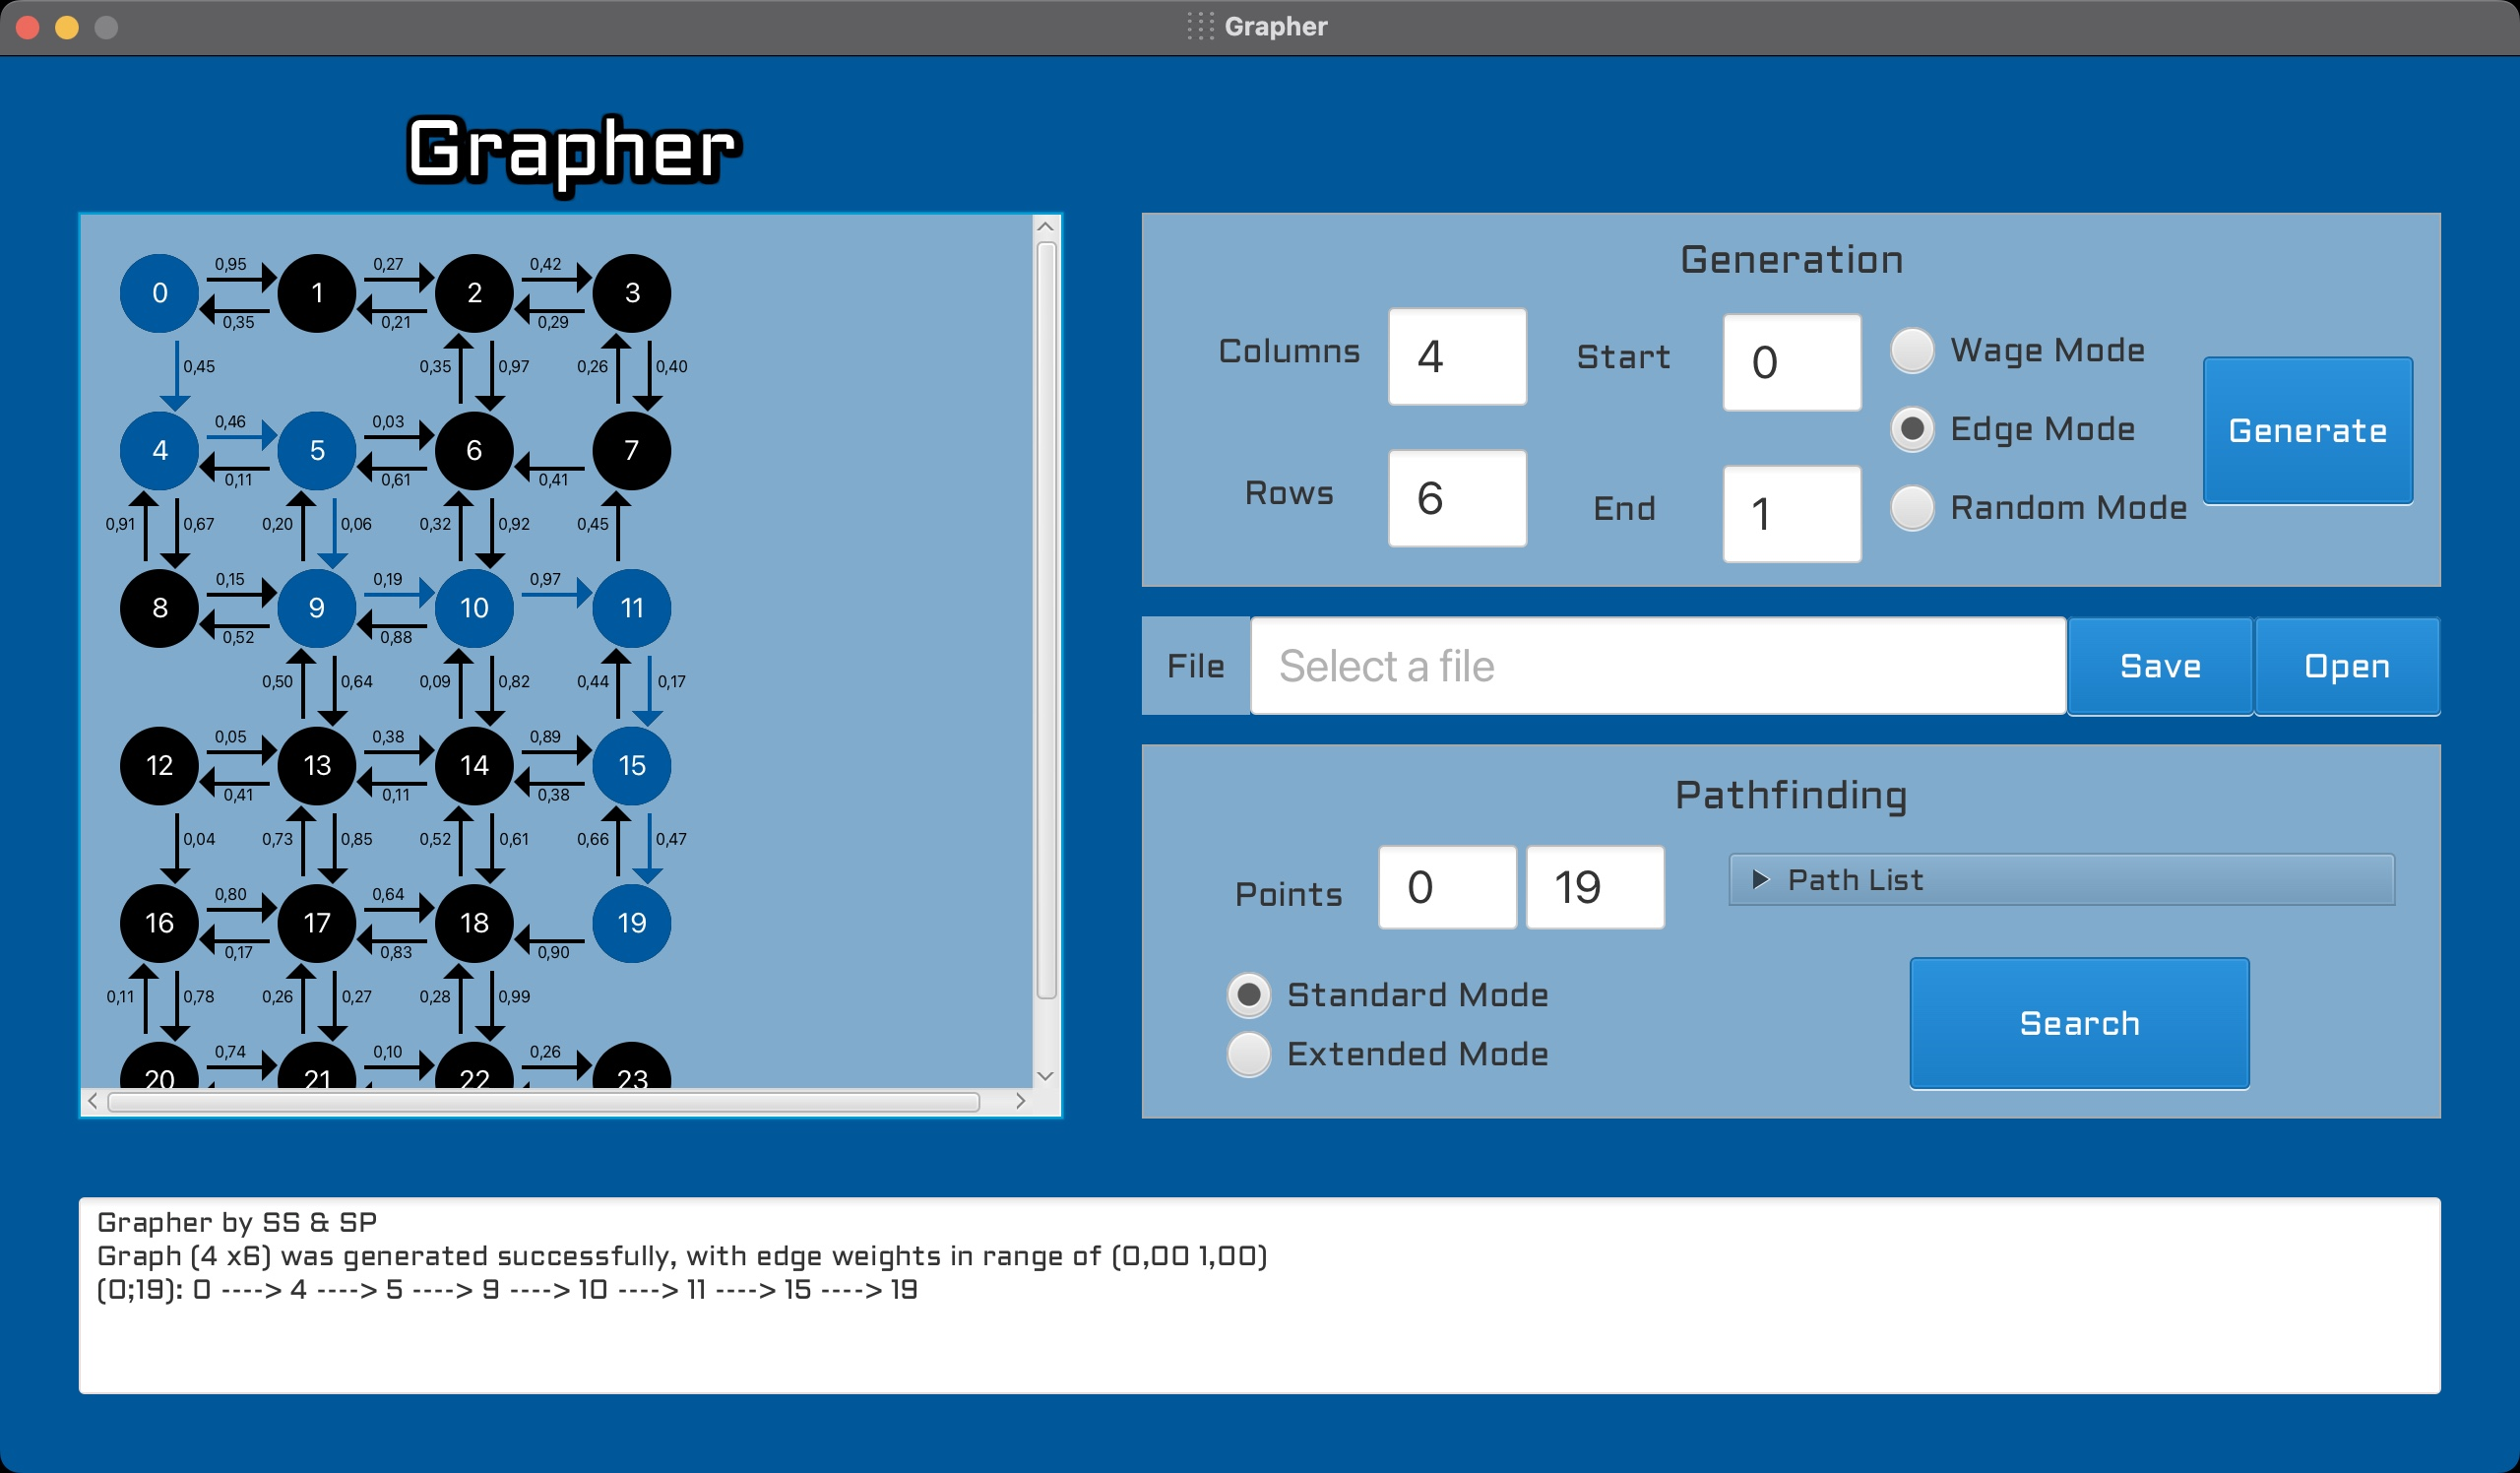
\includegraphics[scale=0.165]{grapherEdgeModePathFinding.jpg}
    \caption{Przykładowe wyszukiwanie najkrótszej ścieżki między punktami w
      grafie typu EdgeMode}
  \end{center}
\end{figure}
\newpage

\subsection{Tryb RandomMode}\label{subsec:random-mode}
Przedstawiamy tryb RandomMode, którego działanie wyjaśnialiśmy wyżej.

\begin{figure}[h]
  \begin{center}
    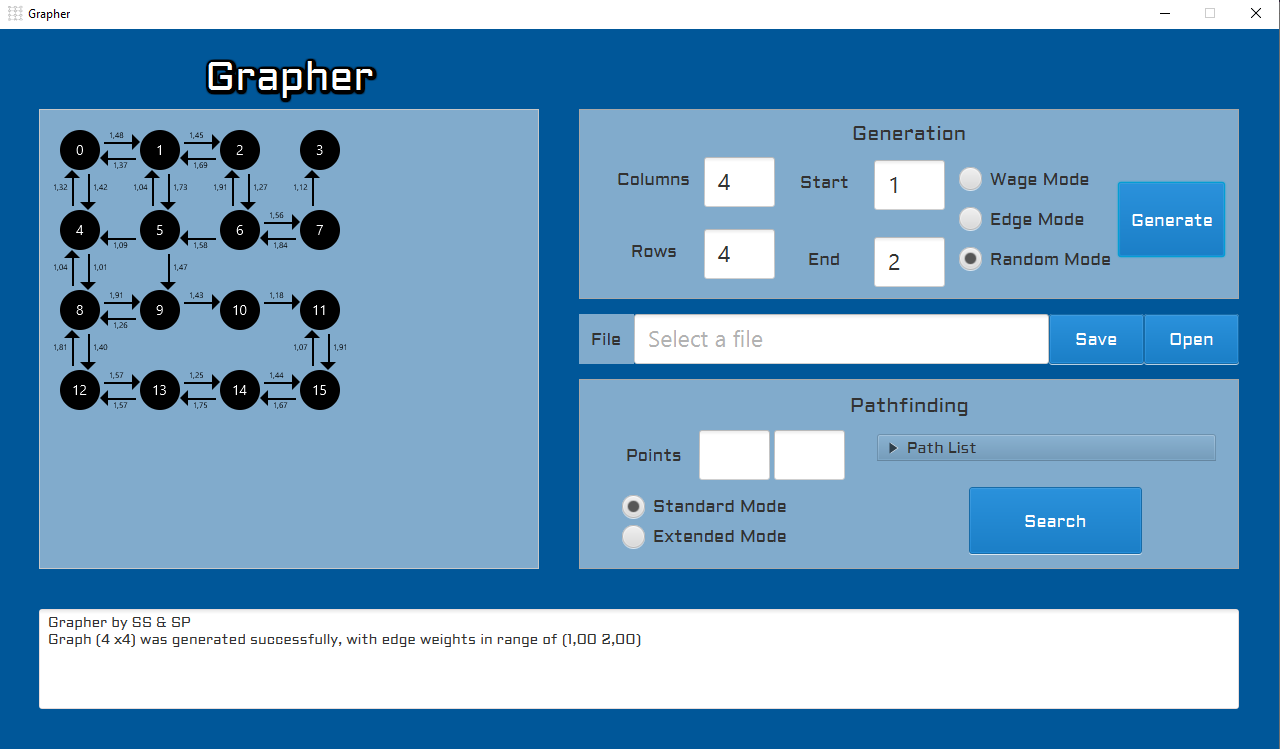
\includegraphics[scale=0.4]{random.png}
    \caption{Wywołanie dla trybu RandomMode.}
  \end{center}
\end{figure}

Program generuje graf i wyświetla go w lewym panelu oraz wyświetla wpis w konsoli o jego pomyślnym wygenerowaniu.
\newpage

\subsection{Zapisywanie grafu}\label{subsec:zapisywanie}
Poniżej pokazujemy zapisywanie wygenerowanego grafu do pliku.

\begin{figure}[h]
  \begin{center}
    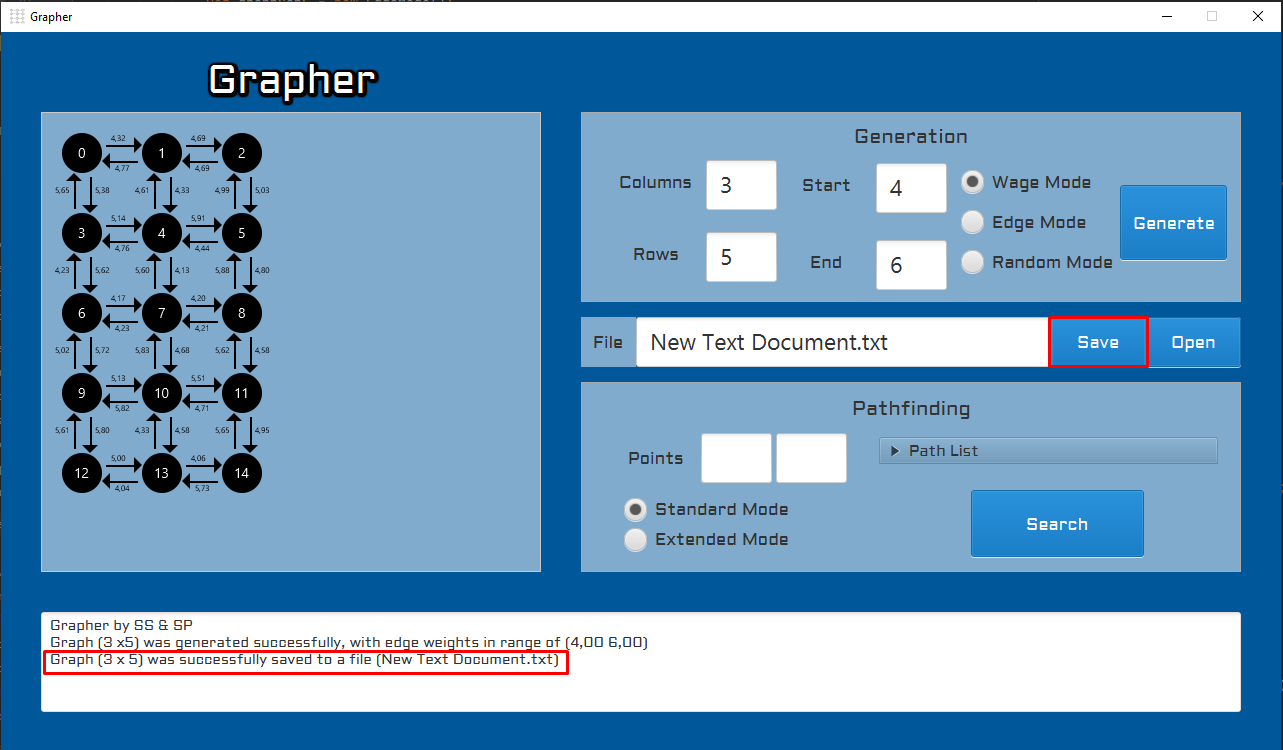
\includegraphics[scale=0.4]{saving.png}
    \caption{Zapisywanie grafu do pliku.}
  \end{center}
\end{figure}
Po kliknięciu przycisku save i wybraniu pliku graf zostaje do niego zapisany i jest to udokumentowane w konsoli.
\newpage

\subsection{Wczytywanie grafu}\label{subsec:wczytywanie}
Tutaj przedstawiamy działanie wczytywanie grafu z pliku.

\begin{figure}[h]
  \begin{center}
    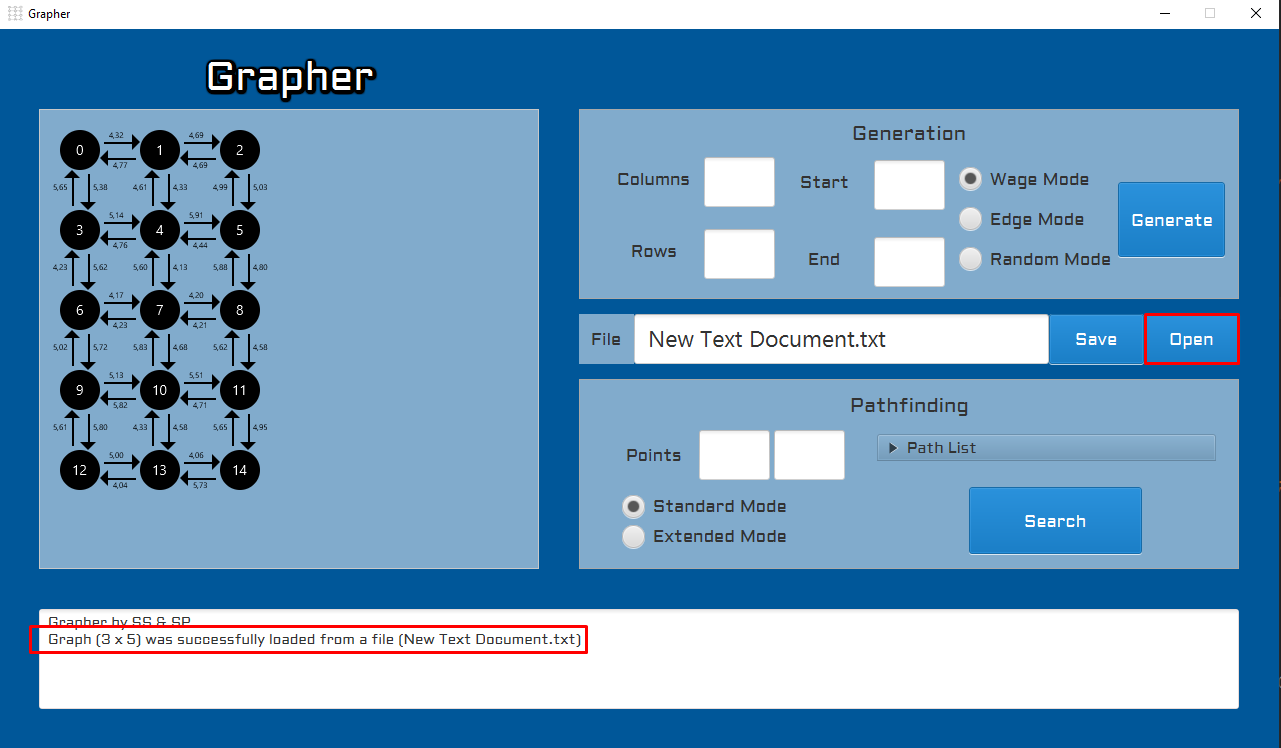
\includegraphics[scale=0.4]{loading.png}
    \caption{Wczytywanie grafu z pliku.}
  \end{center}
\end{figure}
Po wybraniu pliku z grafem o odpowiednim formacie zostaje on wyświetlony w lewym oknie w zależności od jego wielkości.

\newpage

\section{Przeprowadzone testy}\label{sec:przeprowadzone-testy}
Program został przetestowany za pomocą testów wykonanych przy pomocy
\textit{JUnit}. Testy można uruchomić za pomocą \textit{Maven'a} albo przy
pomocy narzędzi programistycznych wbudowanych w odpowiedni IDE.
Przetestowaliśmy wszystkie istotne metody naszego programu i jego wszelkie
zachowania.

\section{Zmiany względem specyfikacji}\label{sec:zmiany-względem-specyfikacji}
W niniejszym rozdziale prezentujemy zmiany, jakie wprowadziliśmy względem tego,
co pojawiło się w specyfikacjach.

\subsection{Klasy i Diagram klas}\label{subsec:klasy-i-diagram-klas}
W trakcie implementacji naszego programu postanowiliśmy zmienić strukturę klas,
a co za tym idzie całego diagramu. W rozdziale poświęconemu strukturze programu
przedstawiliśmy nowy diagram klas.
Tutaj przedstawimy zmiany w klasach.
\begin{itemize}
  \item EntryData -- klasa otrzymała parametr odpowiedzialny za tryb
        wyświetlania ścieżki oraz dodano nowy konstruktor w tejże klasie,
  \item Struktura grafu -- przechowywanie grafu odbywa się teraz za pomocą klas
        Graph i Vertex, a nie jak wcześniej Graph, Vertex, Weights, Connections,
        Existence,
  \item Nazewnictwo nodes -- wszystkie nazwy \textit{nodes} zostały zmienione
        na \textit{vertex},
  \item Klasa GraphIO -- owa klasa została rozbita na dwie mniejsze, czyli
        \textit{GraphReader} i \textit{GraphSaver},
  \item Metoda getpath -- ta metoda została w pełni usunięta,
  \item readFromFile -- metoda teraz zwraca wczytany graf, a nie przyjmuje, tak
        jak to robiła wcześniej, co poskutkowało zmianą typu z \textit{void} na
        \textit{Graph},
  \item Generacja -- klasa ta została usunięte tak samo RandomMode, ponieważ
        uznaliśmy, że domyślnym trybem jest tryb Random, a Edge i Wage są jego
        specjalizacją. Postanowiliśmy wykorzystać tutaj interfejs Generator, z którym
        są zgodne te klasy dziedzicząc po trybie Random implementującym go,
  \item makeConnectionFromVertex -- metoda posiada teraz dostęp do obiekt klasy
        EntryData, czyli userData.
  \item Reszta zmian w klasach -- wszystkie klasy staraliśmy się jak
        najbardziej podzielić klasy żeby podzielić odpowiedzialność na mniejsze klasy
        niż na kilka bardzo dużych.
\end{itemize}

\subsection{Obsługa błędów}\label{subsec:obsługa-błędów}
W naszej specyfikacji implementacyjnej pokazaliśmy tabelę konkretnych błędów
obsługiwanych przez nasz program. Ostatecznie postanowiliśmy z nich
zrezygnować, ponieważ wyjątki obsługiwane w javie okazały się lepszym
sposobem obsługiwania błędów. Wszelkie błędy są obsługiwane za pomocą wyjątków
Javy oraz pokazują się odpowiednie komunikaty w graficznym interfejsie
użytkownika.

\subsection{Testowanie programu}\label{subsec:testowanie-programu}
W specyfikacji napisaliśmy o wykorzystaniu biblioteki \textit{AssertJ} ale
ostatecznie framework \textit{JUnit} zaspokoił w pełni nasze potrzeby związane
z testowaniem.

\subsection{Cel projektu}\label{subsec:cel-projektu}
Usunęliśmy tryb \textit{Read Mode}, ponieważ nie jest on potrzebny jako tryb w naszej aplikacji w Javie dzięki możliwości załączania plików.

\section{Podsumowanie współpracy}\label{sec:podsumowanie-współpracy}
Współpraca podczas projektu obyła się bez znaczących problemów oraz przebiegała
efektywnie.
Dzięki ciągłemu kontaktowi mogliśmy dyskutować nasze pomysły na zmiany
działania programu oraz jego wyglądu.
W kontrolowaniu zmian pomagał nam system kontroli wersji \textit{git}, który
pomagał na bezproblemową pracę z repozytorium oraz wprowadzanie w nim zmian.

\section{Podsumowanie Projektu}\label{sec:podsumowanie-projektu}
Projekt \textit{grapher} był realizowany od 14.04.2022r do 02.06.2022r. W
ramach jego powstała dokumentacja projektu, czyli
specyfikacja funkcjonalna, implementacja oraz niniejsze sprawozdanie.
Oczywiście powstał również sam projekt, który posiada graficzny interfejs
uzytkownika.
Program umożliwia generowanie grafu w trzech trybach oraz czytanie grafu z
możliwością szukania najkrótszej ścieżki między wierzchołkami zadanymi przez
użytkownika.
Sam sposób wyświetlania ścieżki działa w dwóch trybach jeden pokazuje samą
ścieżkę, a drugi pokazuje wagę przejść między wierzchołkami. Program został
przetestowany za pomocą testów
jednostkowych z wykorzystaniem JUnit.

\section{Wnioski}\label{sec:wnioski}
Projekt ten wymagał od nas wiele wysiłku, ponieważ musieliśmy nauczyć się
nowych konceptów takich jak przede wszystkim
programowanie obiektowe. Wymagał on od nas naszej pierwszej pracy z
projektowaniem graficznego interfejsu użytkownika co było dla nas zupełnie
nowym i sporym wyzwaniem.
To samo tyczy się testowania oprogramowania oraz pracy z programem maven,
wymagały one od nas nauki zupełnie nowych technologii i wykorzystanie ich w
projekcie wymagało od nas
szybkiej nauki nowych technologii. Z radością możemy stwierdzić, że wszelkie
problemy związane z tymi rzeczami stały się dla nas przeszłością i dowodem na
to jest w pełni działające
oprogramowanie.

\end{document}